\chapter{Anhang}

\section{Konzept}
    \begin{figure}[htb]
        \centering
        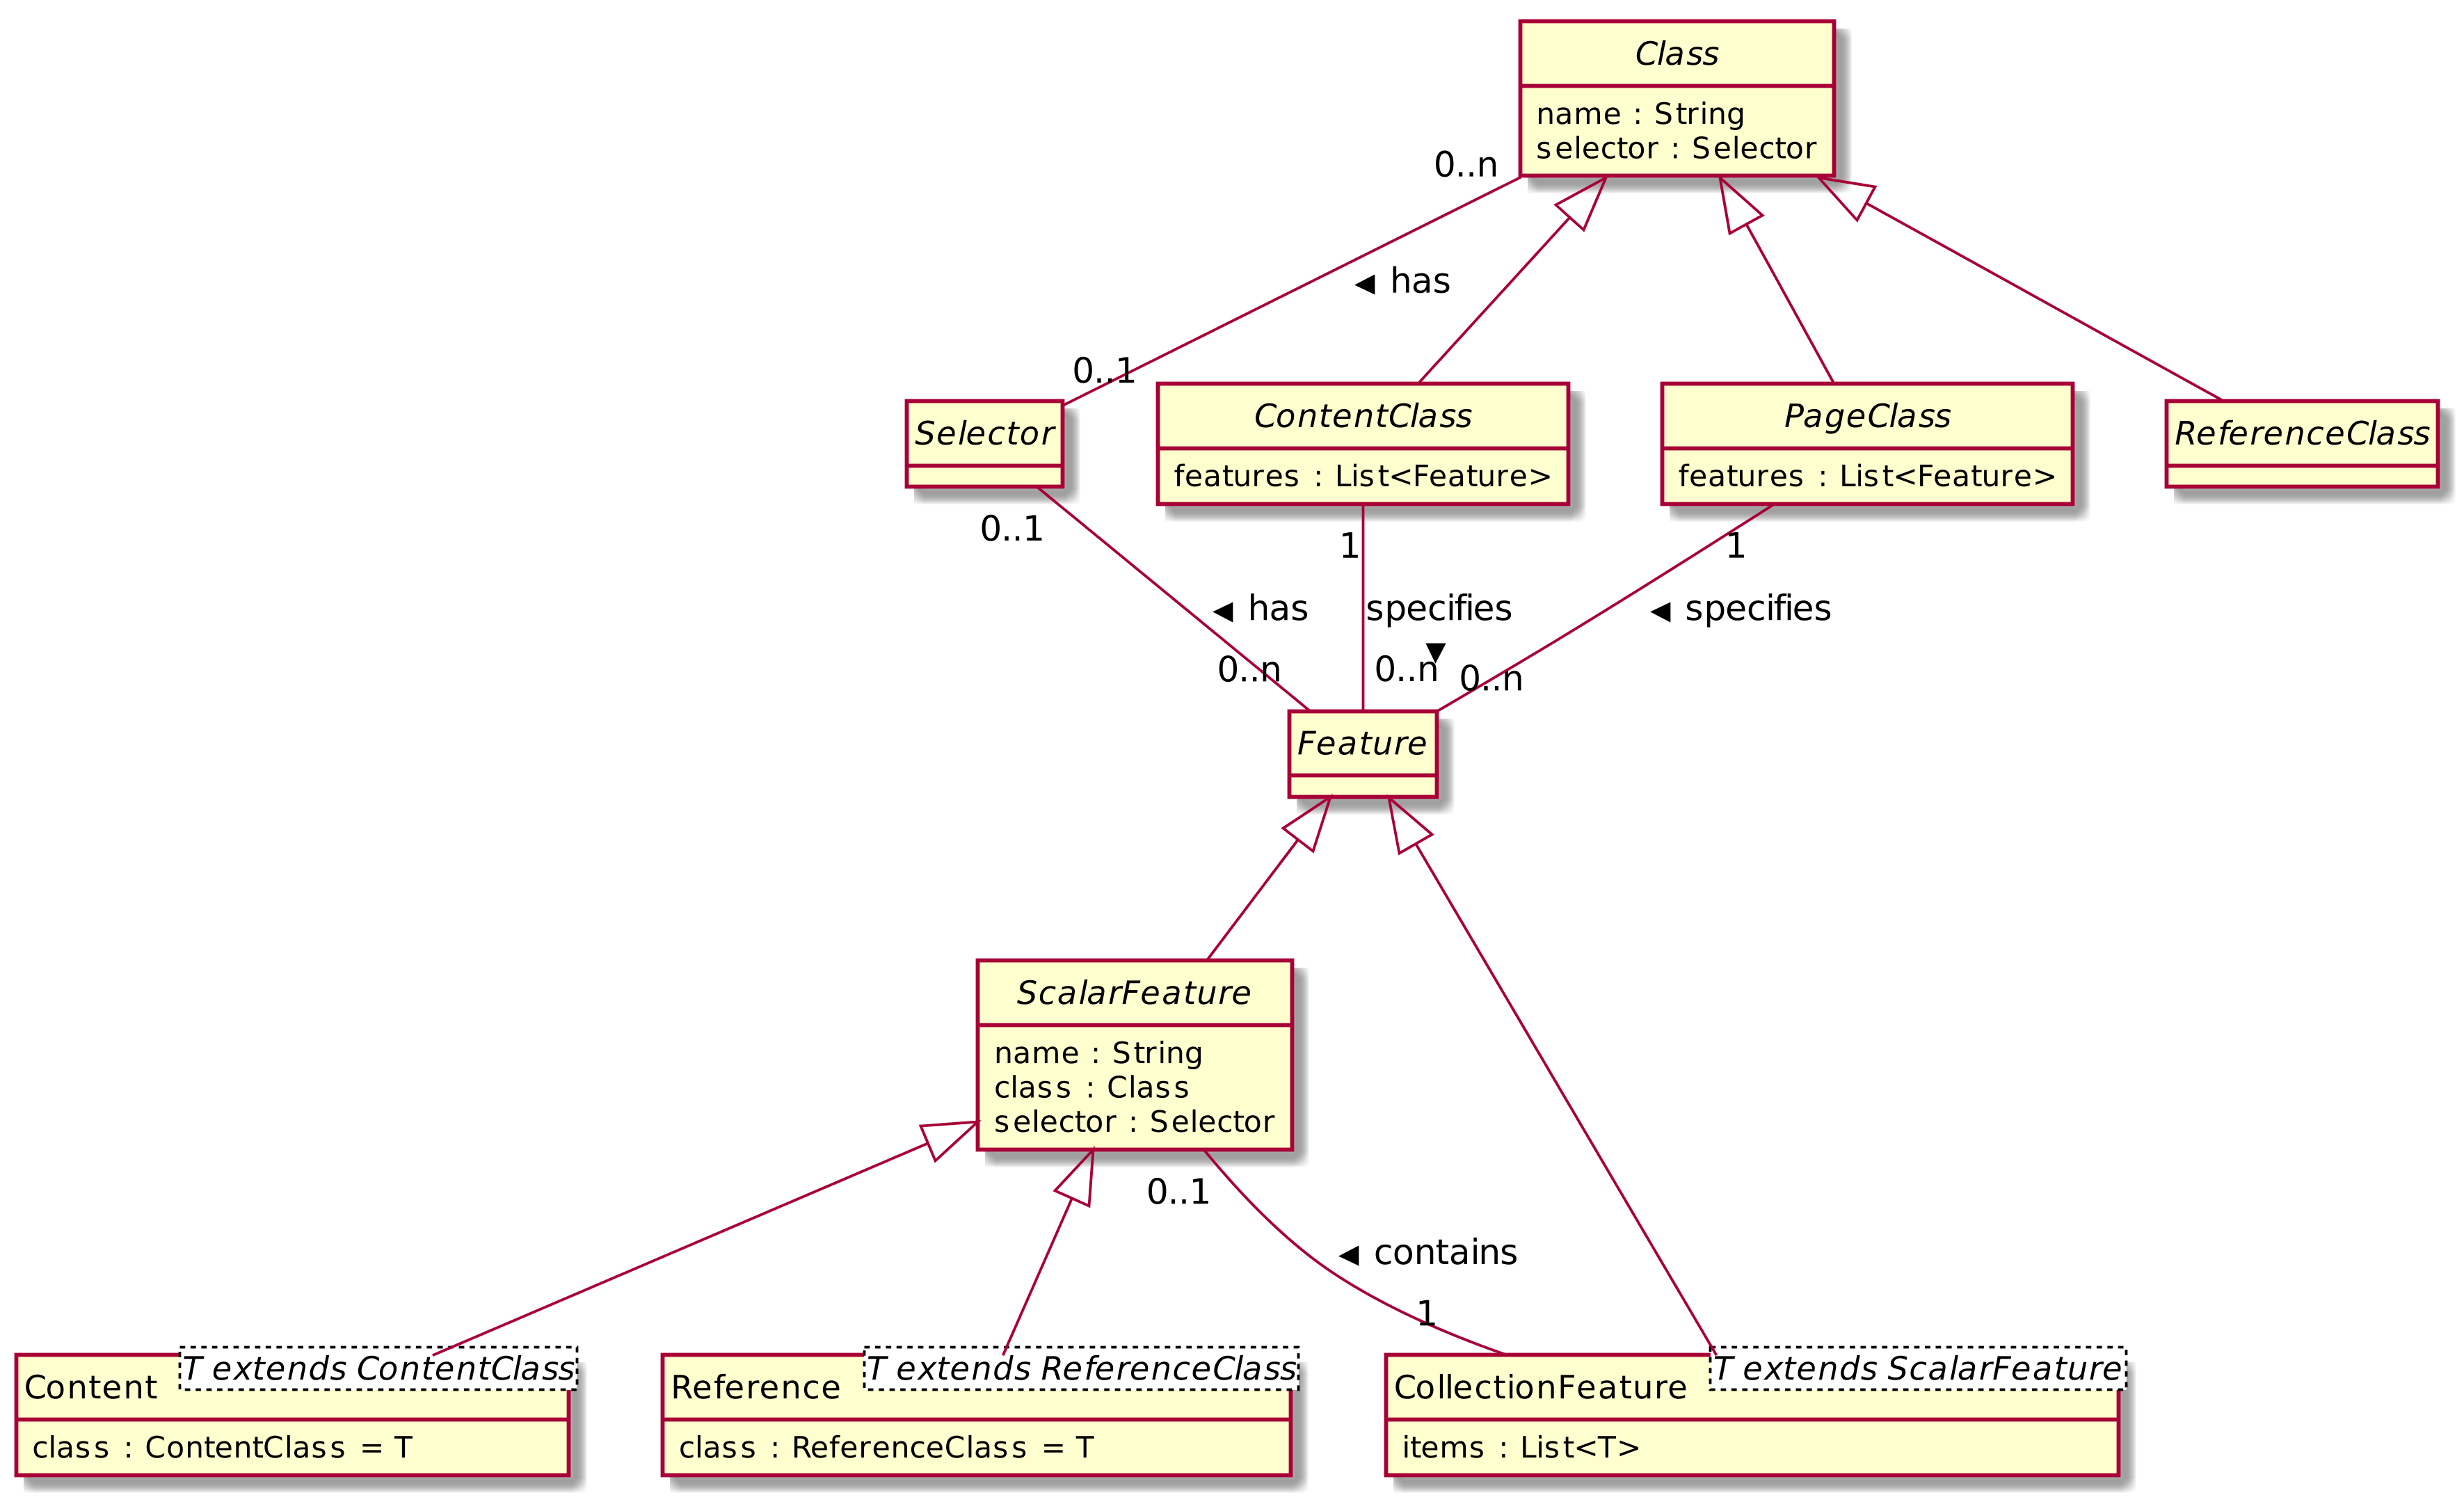
\includegraphics[width=\textwidth]{../resources/concept/classes-features-selectors.png}
        \caption{Klassen, Features, Selektoren}
        \label{image:conceptClassesFeaturesSelectors}
    \end{figure}

\section{Architektur des WCCS}
    Abbildung \ref{image:wccsCompleteArchitecture} zeigt die vollständige Architektur des \glspl{wccs},
    wie sie in Kapitel \ref{section:Architecture} vorgestellt wurde.

    \begin{figure}[htb]
        \centering
        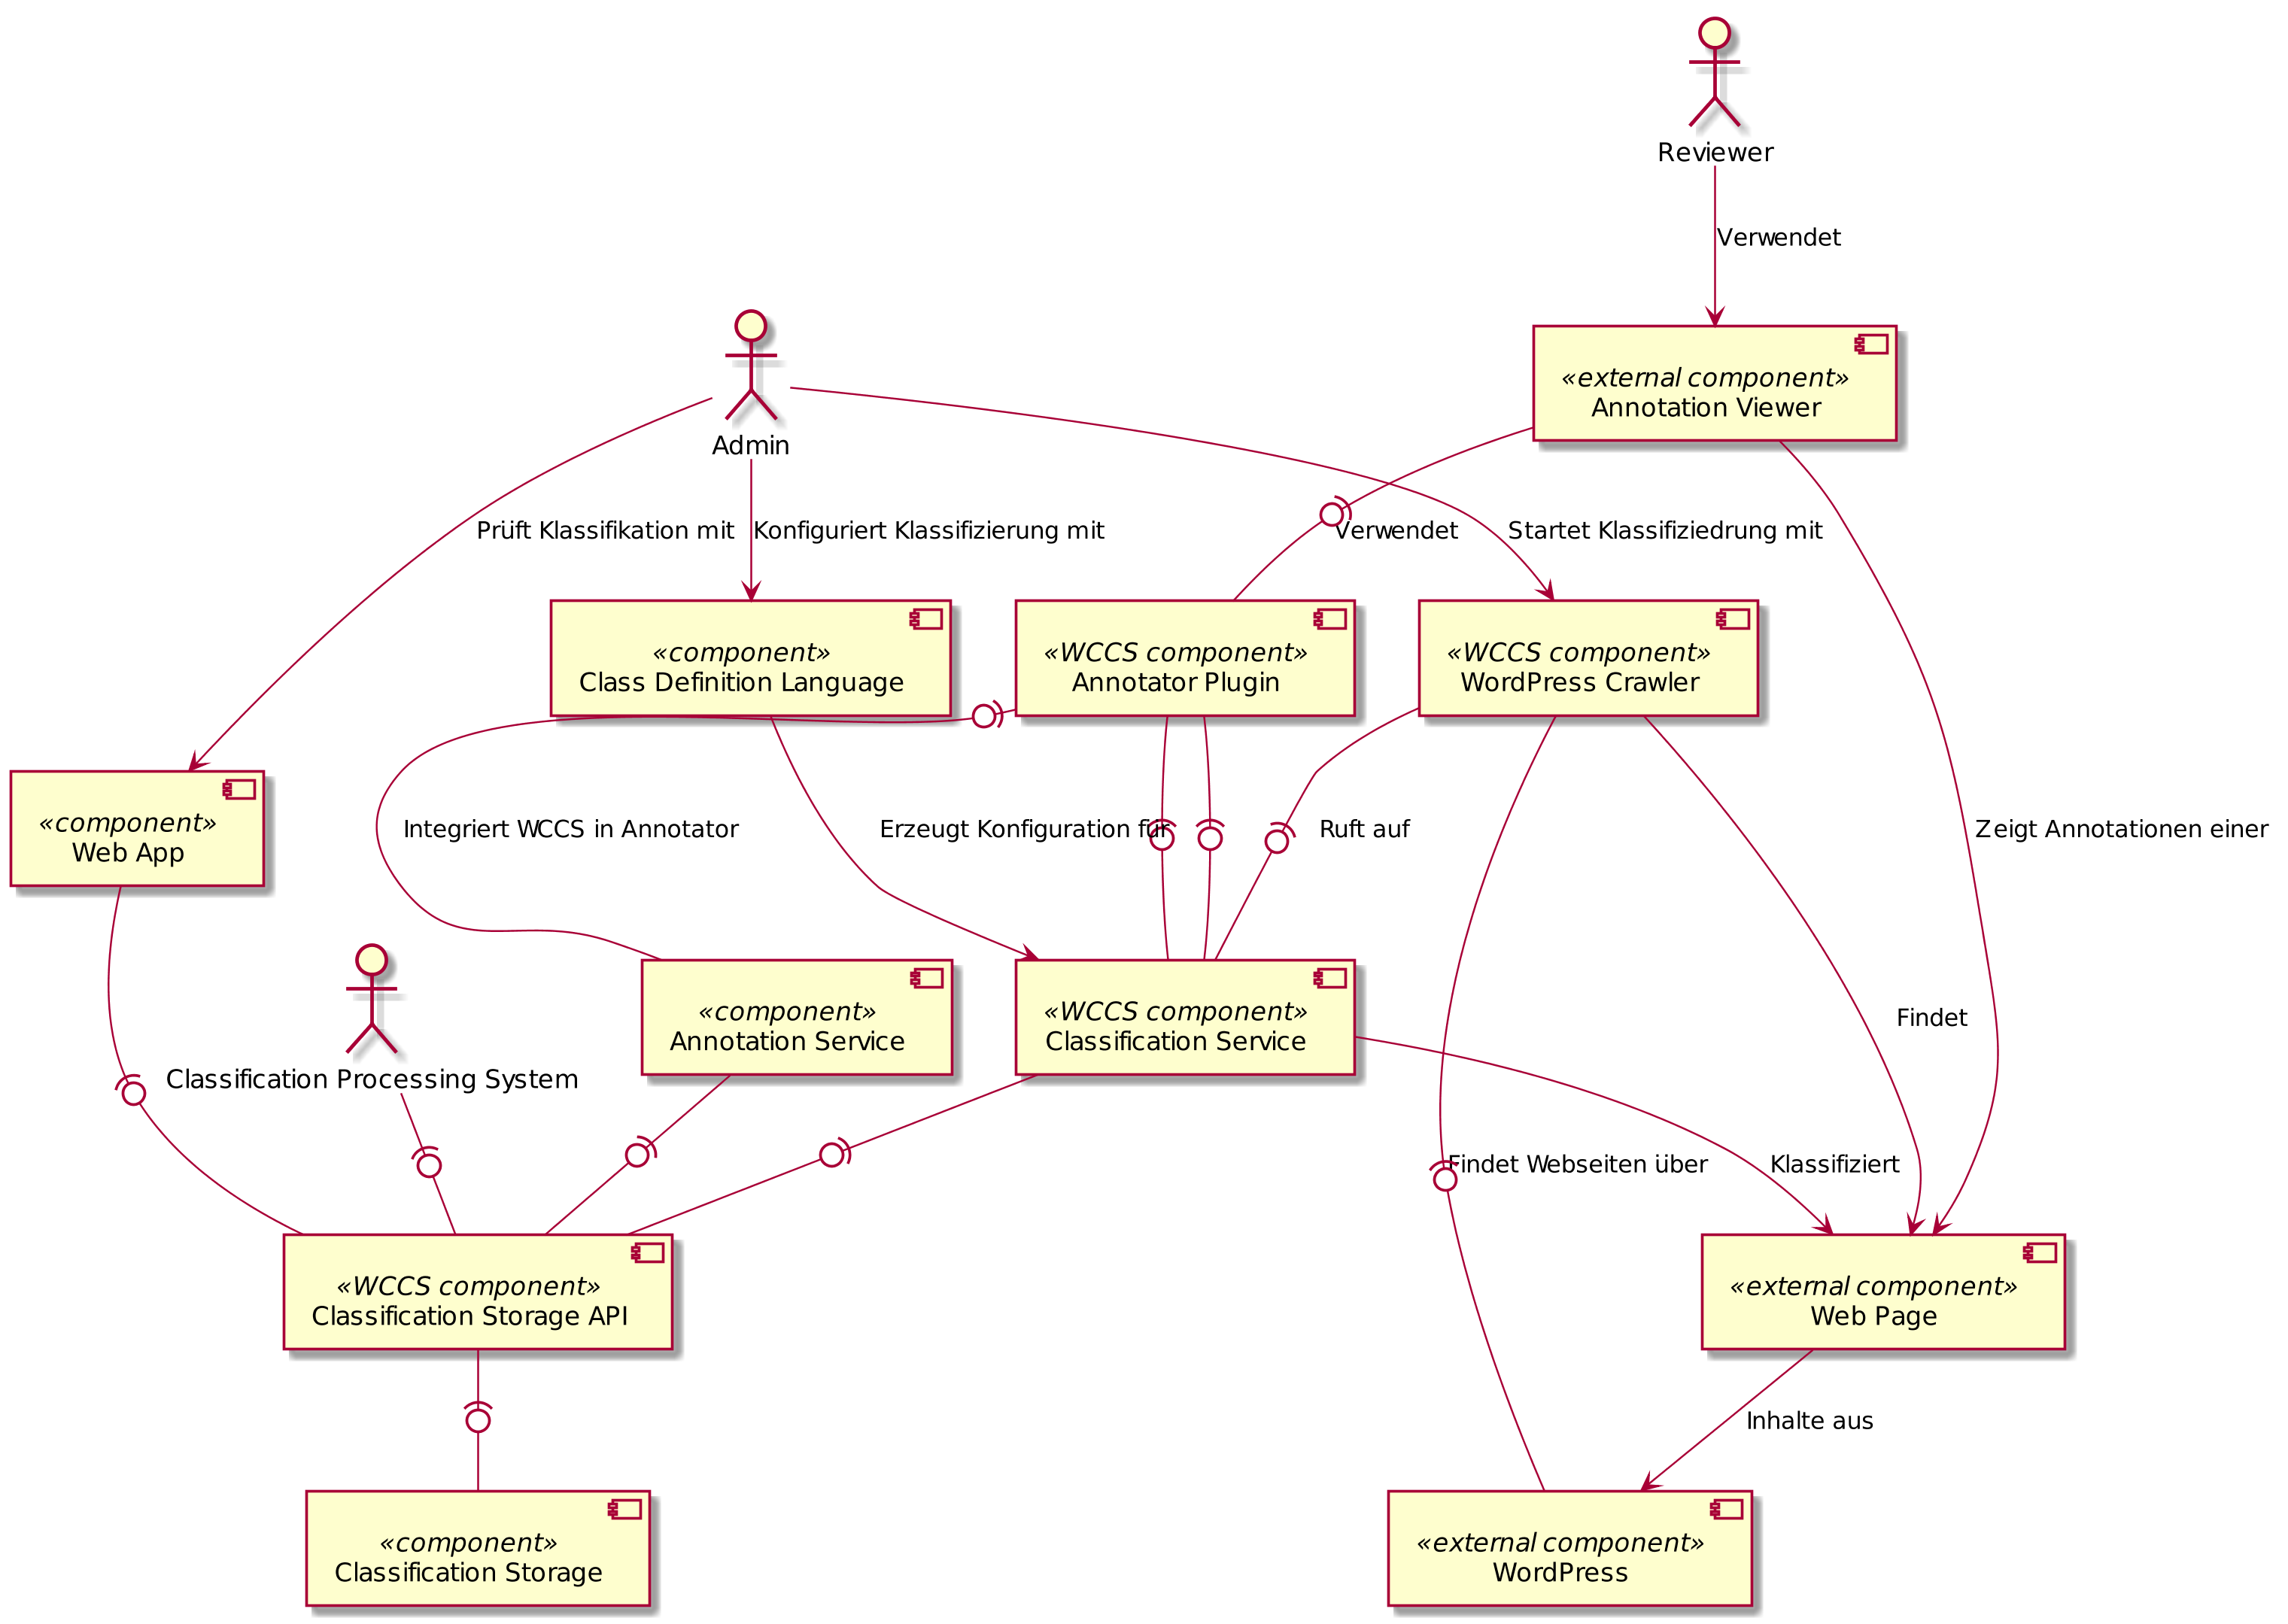
\includegraphics[width=\textwidth]{../resources/architecture/complete_architecture.png}
        \caption{Architkektur des WCCS}
        \label{image:wccsCompleteArchitecture}
    \end{figure}

\section{DSL}
    \label{appendix:dsl}
    \subsection{Modell}
        \begin{figure}[htb]
            \centering
            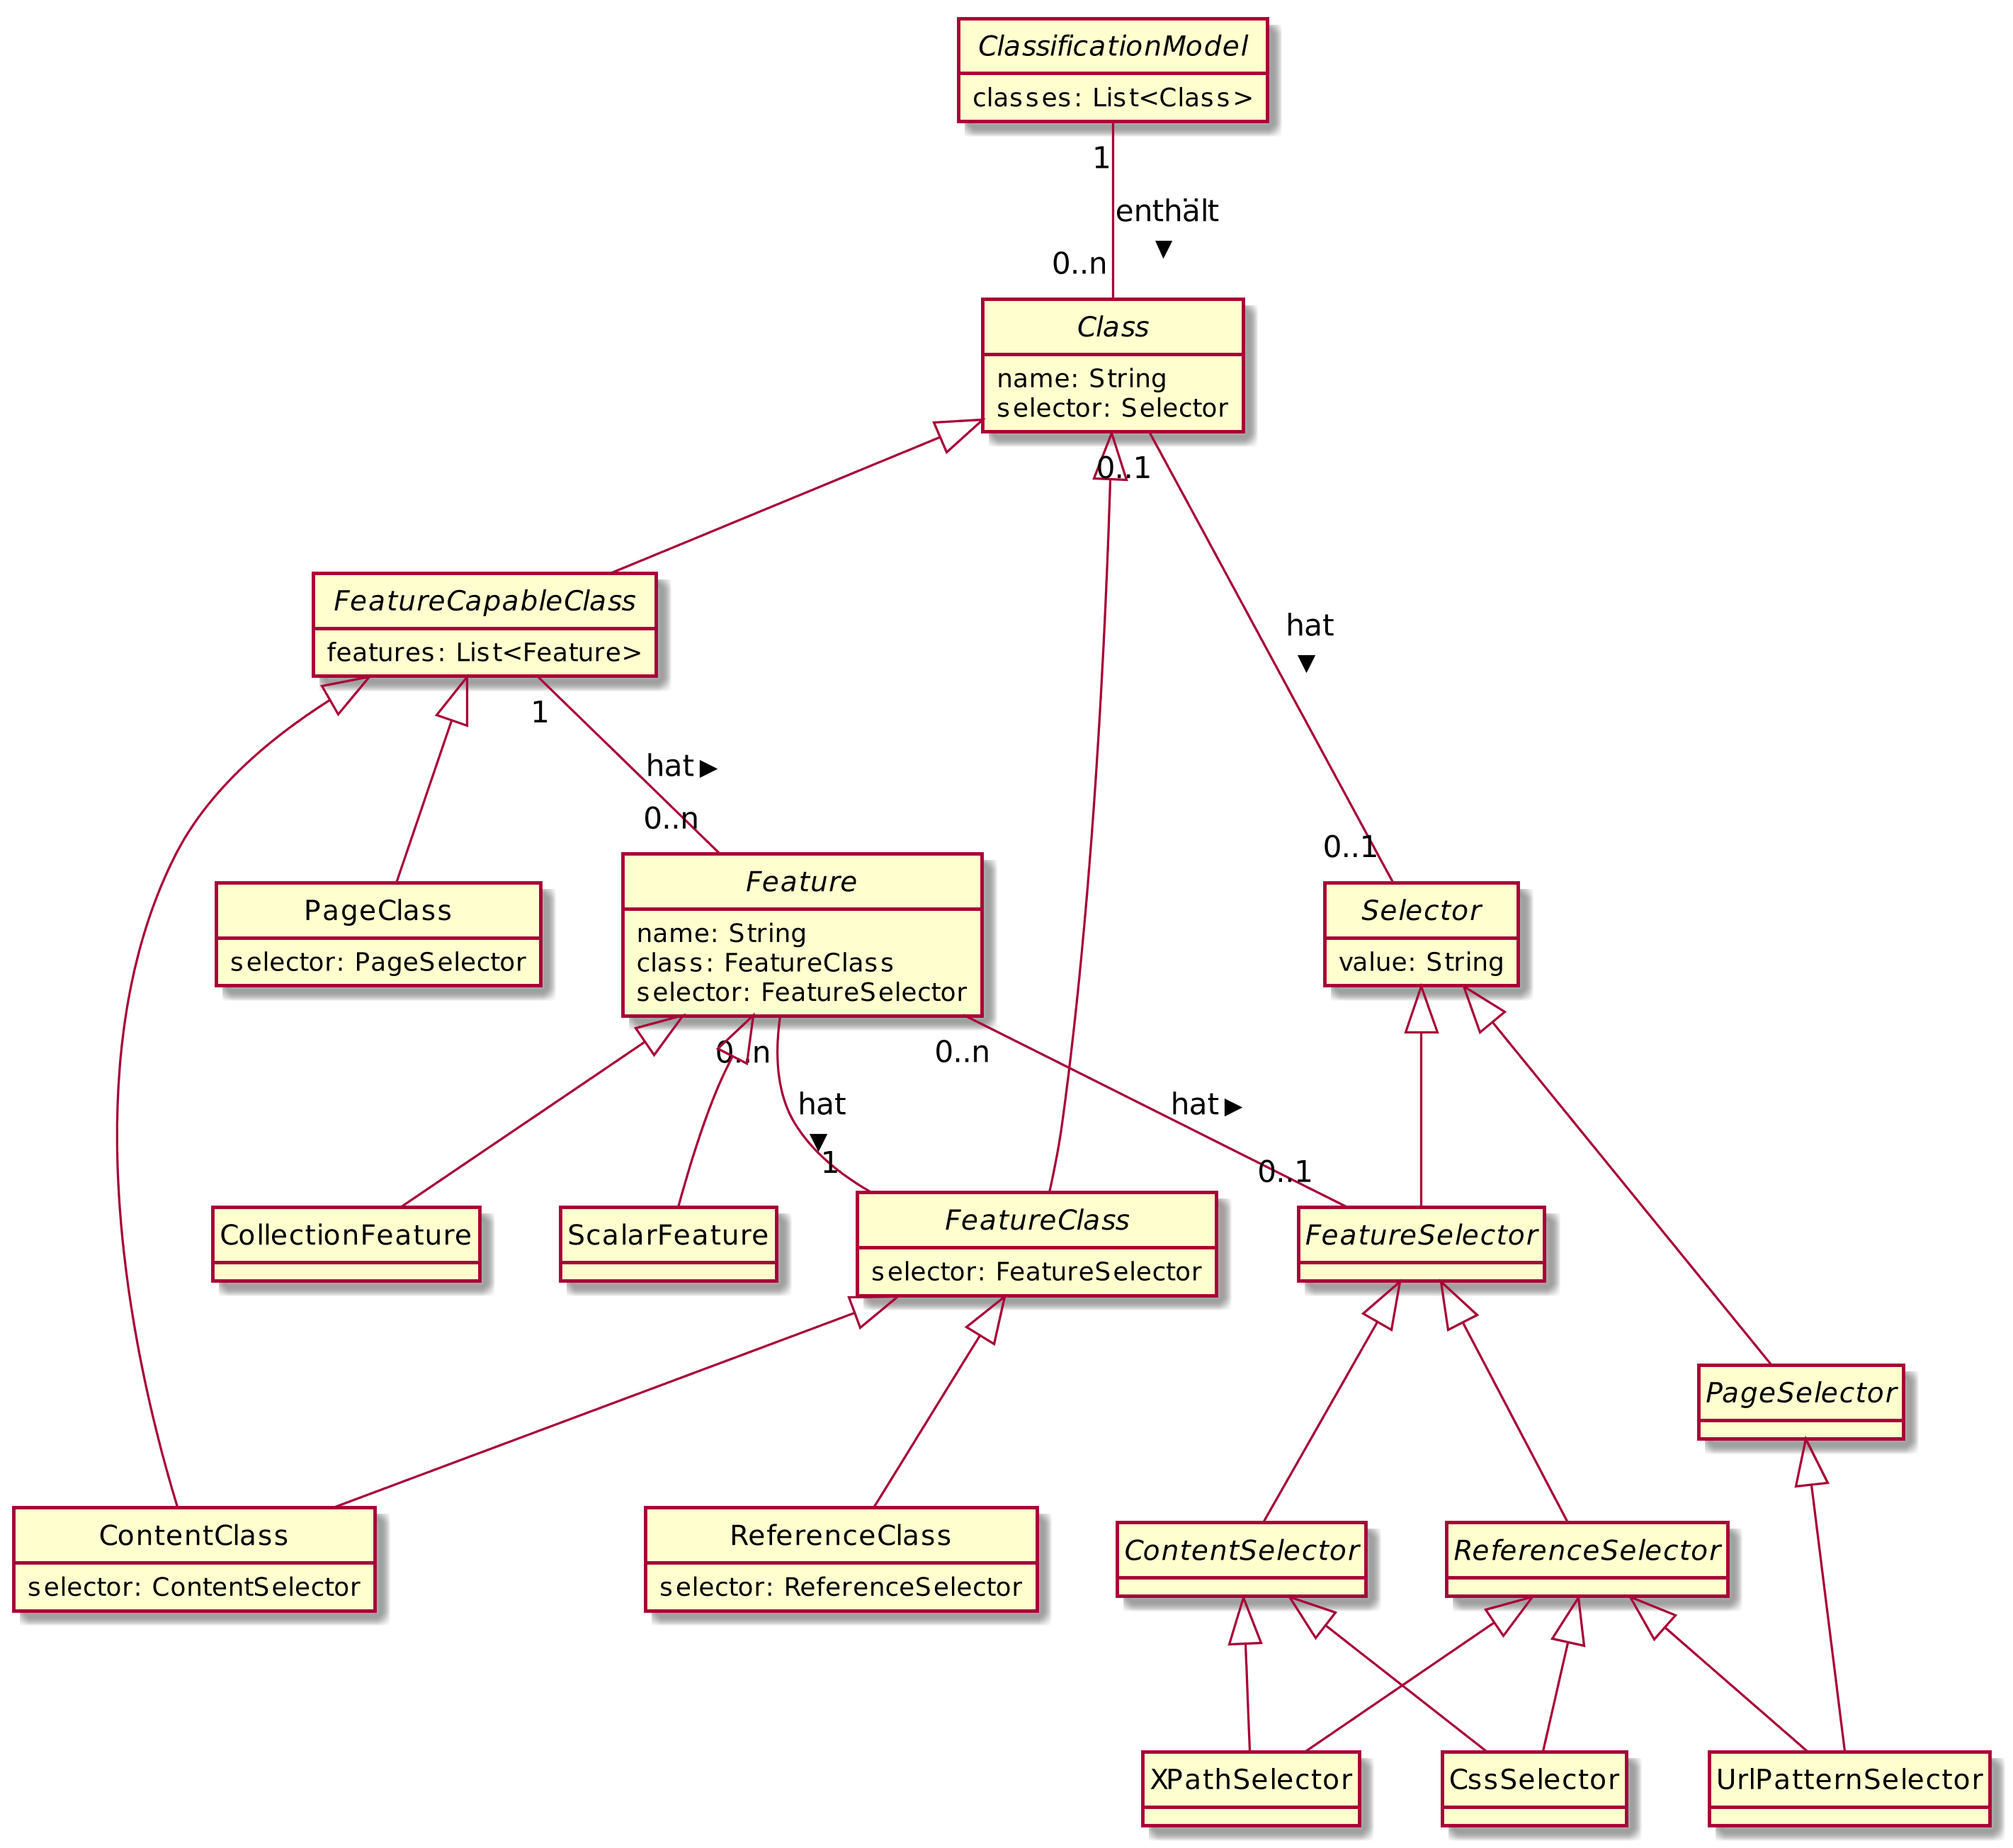
\includegraphics[width=\textwidth]{../resources/dsl/model.png}
            \caption{Modell der DSL}
            \label{image:dslCompleteModel}
        \end{figure}
    
    \subsection{Grammatik}
        \lstinputlisting[
            label=listing:dlsGrammar,
            caption=Grammatik der DSL,
            language=wccdl,
            inputencoding=utf8/latin1]{../resources/dsl/grammar/grammar.xtext}

    \subsection{Transformation}
        \lstinputlisting[
            label=listing:dlsGenerationComplete,
            caption=Vollständiges Generat
        ]{../resources/dsl/generation/complete.json}

\section{Classification Storage API}
    % TODO: Braucht man das überhaupt?
    \lstinputlisting[
        label=listing:storeClassification,
        caption=Vollständiger Algorithmus zum Speichern einer Seite,
        style=pseudo
    ]{../resources/classification-storage-api/store-classification-alg/complete.code}